\iffalse
\let\negmedspace\undefined
\let\negthickspace\undefined
\documentclass[journal,12pt,twocolumn]{IEEEtran}
\usepackage{cite}
\usepackage{amsmath,amssymb,amsfonts,amsthm}
\usepackage{algorithmic}
\usepackage{graphicx}
\usepackage{textcomp}
\usepackage{xcolor}
\usepackage{txfonts}
\usepackage{listings}
\usepackage{enumitem}
\usepackage{mathtools}
\usepackage{gensymb}
\usepackage[breaklinks=true]{hyperref}
\usepackage{tkz-euclide} % loads  TikZ and tkz-base
\usepackage{listings}
\usepackage{float}

%
%\usepackage{setspace}
%\usepackage{gensymb}
%\doublespacing
%\singlespacing

\usepackage{graphicx}
%\usepackage{amssymb}
%\usepackage{relsize}
%\usepackage[cmex10]{amsmath}
%\usepackage{amsthm}
%\interdisplaylinepenalty=2500
%\savesymbol{iint}
%\usepackage{txfonts}
%\restoresymbol{TXF}{iint}
%\usepackage{wasysym}
%\usepackage{amsthm}
%\usepackage{iithtlc}
%\usepackage{mathrsfs}
%\usepackage{txfonts}
%\usepackage{stfloats}
%\usepackage{bm}
%\usepackage{cite}
%\usepackage{cases}
%\usepackage{subfig}
%\usepackage{xtab}
%\usepackage{longtable}
%\usepackage{multirow}
%\usepackage{algorithm}
%\usepackage{algpseudocode}
%\usepackage{enumitem}
%\usepackage{mathtools}
%\usepackage{tikz}
%\usepackage{circuitikz}
%\usepackage{verbatim}
%\usepackage{tfrupee}
%\usepackage{stmaryrd}
%\usetkzobj{all}
%    \usepackage{color}                                            %%
%    \usepackage{array}                                            %%
%    \usepackage{longtable}                                        %%
%    \usepackage{calc}                                             %%
%    \usepackage{multirow}                                         %%
%    \usepackage{hhline}                                           %%
%    \usepackage{ifthen}                                           %%
  %optionally (for landscape tables embedded in another document): %%
%    \usepackage{lscape}     
%\usepackage{multicol}
%\usepackage{chngcntr}
%\usepackage{enumerate}

%\usepackage{wasysym}
%\documentclass[conference]{IEEEtran}
%\IEEEoverridecommandlockouts
% The preceding line is only needed to identify funding in the first footnote. If that is unneeded, please comment it out.

\newtheorem{theorem}{Theorem}[section]
\newtheorem{problem}{Problem}
\newtheorem{proposition}{Proposition}[section]
\newtheorem{lemma}{Lemma}[section]
\newtheorem{corollary}[theorem]{Corollary}
\newtheorem{example}{Example}[section]
\newtheorem{definition}[problem]{Definition}
%\newtheorem{thm}{Theorem}[section] 
%\newtheorem{defn}[thm]{Definition}
%\newtheorem{algorithm}{Algorithm}[section]
%\newtheorem{cor}{Corollary}
\newcommand{\BEQA}{\begin{eqnarray}}
\newcommand{\EEQA}{\end{eqnarray}}
\newcommand{\define}{\stackrel{\triangle}{=}}
\theoremstyle{remark}
\newtheorem{rem}{Remark}
\parindent 0px

%\bibliographystyle{ieeetr}
\begin{document}
%
\providecommand{\pr}[1]{\ensuremath{\Pr\left(#1\right)}}
\providecommand{\prt}[2]{\ensuremath{p_{#1}^{\left(#2\right)} }}        % own macro for this question
\providecommand{\qfunc}[1]{\ensuremath{Q\left(#1\right)}}
\providecommand{\sbrak}[1]{\ensuremath{{}\left[#1\right]}}
\providecommand{\lsbrak}[1]{\ensuremath{{}\left[#1\right.}}
\providecommand{\rsbrak}[1]{\ensuremath{{}\left.#1\right]}}
\providecommand{\brak}[1]{\ensuremath{\left(#1\right)}}
\providecommand{\lbrak}[1]{\ensuremath{\left(#1\right.}}
\providecommand{\rbrak}[1]{\ensuremath{\left.#1\right)}}
\providecommand{\cbrak}[1]{\ensuremath{\left\{#1\right\}}}
\providecommand{\lcbrak}[1]{\ensuremath{\left\{#1\right.}}
\providecommand{\rcbrak}[1]{\ensuremath{\left.#1\right\}}}
\newcommand{\sgn}{\mathop{\mathrm{sgn}}}
\providecommand{\abs}[1]{\left\vert#1\right\vert}
\providecommand{\res}[1]{\Res\displaylimits_{#1}} 
\providecommand{\norm}[1]{\left\lVert#1\right\rVert}
%\providecommand{\norm}[1]{\lVert#1\rVert}
\providecommand{\mtx}[1]{\mathbf{#1}}
\providecommand{\mean}[1]{E\left[ #1 \right]}
\providecommand{\cond}[2]{#1\middle|#2}
\providecommand{\fourier}{\overset{\mathcal{F}}{ \rightleftharpoons}}
\newenvironment{amatrix}[1]{%
  \left(\begin{array}{@{}*{#1}{c}|c@{}}
}{%
  \end{array}\right)
}
%\providecommand{\hilbert}{\overset{\mathcal{H}}{ \rightleftharpoons}}
%\providecommand{\system}{\overset{\mathcal{H}}{ \longleftrightarrow}}
	%\newcommand{\solution}[2]{\textbf{Solution:}{#1}}
\newcommand{\solution}{\noindent \textbf{Solution: }}
\newcommand{\cosec}{\,\text{cosec}\,}
\providecommand{\dec}[2]{\ensuremath{\overset{#1}{\underset{#2}{\gtrless}}}}
\newcommand{\myvec}[1]{\ensuremath{\begin{pmatrix}#1\end{pmatrix}}}
\newcommand{\mydet}[1]{\ensuremath{\begin{vmatrix}#1\end{vmatrix}}}
\newcommand{\myaugvec}[2]{\ensuremath{\begin{amatrix}{#1}#2\end{amatrix}}}
\providecommand{\rank}{\text{rank}}
\providecommand{\pr}[1]{\ensuremath{\Pr\left(#1\right)}}
\providecommand{\qfunc}[1]{\ensuremath{Q\left(#1\right)}}
	\newcommand*{\permcomb}[4][0mu]{{{}^{#3}\mkern#1#2_{#4}}}
\newcommand*{\perm}[1][-3mu]{\permcomb[#1]{P}}
\newcommand*{\comb}[1][-1mu]{\permcomb[#1]{C}}
\providecommand{\qfunc}[1]{\ensuremath{Q\left(#1\right)}}
\providecommand{\gauss}[2]{\mathcal{N}\ensuremath{\left(#1,#2\right)}}
\providecommand{\diff}[2]{\ensuremath{\frac{d{#1}}{d{#2}}}}
\providecommand{\myceil}[1]{\left \lceil #1 \right \rceil }
\newcommand\figref{Fig.~\ref}
\newcommand\tabref{Table~\ref}
\newcommand{\sinc}{\,\text{sinc}\,}
\newcommand{\rect}{\,\text{rect}\,}
%%
%	%\newcommand{\solution}[2]{\textbf{Solution:}{#1}}
%\newcommand{\solution}{\noindent \textbf{Solution: }}
%\newcommand{\cosec}{\,\text{cosec}\,}
%\numberwithin{equation}{section}
%\numberwithin{equation}{subsection}
%\numberwithin{problem}{section}
%\numberwithin{definition}{section}
%\makeatletter
%\@addtoreset{figure}{problem}
%\makeatother

%\let\StandardTheFigure\thefigure
\let\vec\mathbf


\bibliographystyle{IEEEtran}


\vspace{3cm}

\title{
%	\logo{
%	}
}
\author{Sreeja Komakula - EE22BTECH11029}

	
	

%\title{
%	\logo{Matrix Analysis through Octave}{\begin{center}\includegraphics[scale=.24]{tlc}\end{center}}{}{HAMDSP}
%}


% paper title
% can use linebreaks \\ within to get better formatting as desired
%\title{Matrix Analysis through Octave}
%
%
% author names and IEEE memberships
% note positions of commas and nonbreaking spaces ( ~ ) LaTeX will not break
% a structure at a ~ so this keeps an author's name from being broken across
% two lines.
% use \thanks{} to gain access to the first footnote area
% a separate \thanks must be used for each paragraph as LaTeX2e's \thanks
% was not built to handle multiple paragraphs
%

%\author{<-this % stops a space
%\thanks{}}
%}
% note the % following the last \IEEEmembership and also \thanks - 
% these prevent an unwanted space from occurring between the last author name
% and the end of the author line. i.e., if you had this:
% 
% \author{....lastname \thanks{...} \thanks{...} }
%                     ^------------^------------^----Do not want these spaces!
%
% a space would be appended to the last name and could cause every name on that
% line to be shifted left slightly. This is one of those "LaTeX things". For
% instance, "\textbf{A} \textbf{B}" will typeset as "A B" not "AB". To get
% "AB" then you have to do: "\textbf{A}\textbf{B}"
% \thanks is no different in this regard, so shield the last } of each \thanks
% that ends a line with a % and do not let a space in before the next \thanks.
% Spaces after \IEEEmembership other than the last one are OK (and needed) as
% you are supposed to have spaces between the names. For what it is worth,
% this is a minor point as most people would not even notice if the said evil
% space somehow managed to creep in.



% The paper headers
%\markboth{Journal of \LaTeX\ Class Files,~Vol.~6, No.~1, January~2007}%
%{Shell \MakeLowercase{\textit{et al.}}: Bare Demo of IEEEtran.cls for Journals}
% The only time the second header will appear is for the odd numbered pages
% after the title page when using the twoside option.
% 
% *** Note that you probably will NOT want to include the author's ***
% *** name in the headers of peer review papers.                   ***
% You can use \ifCLASSOPTIONpeerreview for conditional compilation here if
% you desire.




% If you want to put a publisher's ID mark on the page you can do it like
% this:
%\IEEEpubid{0000--0000/00\$00.00~\copyright~2007 IEEE}
% Remember, if you use this you must call \IEEEpubidadjcol in the second
% column for its text to clear the IEEEpubid mark.



% make the title area
\maketitle
\textbf{Question 56}\\
Let $(X,Y)$ have joint probability mass function
\begin{align}
p_{XY}\brak{x,y}&=
\begin{cases}
\frac{e^{-2}}{x!(y - x)!} & if x = 0,1,....,y; y = 0,1,2,....\\
0 & otherwise.\\
\end{cases}
\end{align}
Then which of the following statements is/are true?
\begin{enumerate}
\item ${E(X|Y = 4) = 2}$
\item The moment generating function of $Y$ is $e^{2(e^v - 1)}$ for all $v \in R$
\item ${E(X) = 2}$
\item The joint moment generating function of $(X,Y)$ is $e^{-2+(1 + e^u)e^v}$ for all $(u,v) \in {R^2}$
\end{enumerate}
\hfill(GATE ST 2023)\\
\solution
\fi
Given
\begin{align}
p_{XY}\brak{x,y}&=\frac{e^{-2}}{x!(y - x)!}
\end{align}
Then,
\begin{align}
p_Y\brak{y} &= \sum_{x=0}^{\infty}p_{XY}\brak{x,y}dx\\
&= \sum_{x=0}^{\infty} \frac{e^{-2}}{x!(y - x)!}\\
&= \frac{e^{-2}2^y}{y!}\\
\end{align}
\begin{enumerate}
\item ${E(X|Y = 4) = 2}$:
\begin{align}
E\brak{X|Y=4} &= \sum_{x} x\frac{p_{XY}\brak{x,y}}{p_Y\brak{y}}\\
&= \sum_{x=0}^{4} x\frac{p_{XY}\brak{x,4}}{p_Y\brak{4}}\\
&= \sum_{x=0}^{4} x\frac{4!}{2^4 x!(4-x)!}\\
&= \sum_{x=0}^{4} x\frac{24}{16 x!(4-x)!}\\
&= \sum_{x=0}^{4} x\frac{3}{2 x!(4-x)!}\\
&= \frac{3}{2}(0 + \frac{1}{6} + \frac{1}{2} + \frac{1}{2} + \frac{1}{6})\\
&= \frac{3}{2}\times \frac{4}{3}\\
&= 2
\end{align}
Hence, the given statement is true.
\item The moment generating function of $Y$ is $e^{2(e^v - 1)}$ for all $v \in R$:\\
The $z$-transform of $Y$ is defined as:
\begin{align}
M_Y\brak{z} &= E\sbrak{z^{-y}}\\
&= \sum_{k=0}^{\infty} p_Y\brak{k}z^{-k}\\
&= \sum_{k=0}^{\infty} \frac{e^{-2}2^k}{k!}z^{-k}\\
&= e^{-2} \sum_{k=0}^{\infty} \frac{z^{-k}2^k}{k!}\\
&= e^{-2} \sum_{k=0}^{\infty} \frac{(\frac{2}{z})^k}{k!}\\
&= e^{-2+\frac{2}{z}}
\end{align}
For moment generating function, $z$ is replaced by $e^{-z}$, we get
\begin{align}
M_Y\brak{z} &= e^{-2+\frac{2}{e^{-z}}}\\
&= e^{-2+2e^z}\\
&= e^{2(e^z-1)}\\
\implies M_Y\brak{v} = e^{2(e^v-1)} 
\end{align}
Hence, the given statement is true.
\item ${E(X) = 2}$:
\begin{align}
p_X\brak{x} &= \sum_{y=x}^{\infty}p_{XY}\brak{x,y}dy\\
&= \sum_{y=x}^{\infty} \frac{e^{-2}}{x!(y - x)!}\\
&= \frac{e^{-2}}{x!}\sum_{y=x}^{\infty}\frac{1}{(y - x)!}\\
&= \frac{e^{-2}e}{x!}\\
&= \frac{e^{-1}}{x!}
\end{align}
Moment generating function is defined as:
\begin{align}
M_X\brak{t} &= E\brak{e^{tx}}\\
&= \sum_{k=0}^{\infty} p_X\brak{k}e^{tk}
\end{align}
In $z$-transform we replace $e^{t}$ with $z^{-1}$.\\
\begin{align}
M_X\brak{\nu} &= E\brak{\nu^{-x}}\\
&= \sum_{k=0}^{\infty} p_X\brak{k}\nu^{-k}\\
&= \sum_{k=0}^{\infty} \frac{e^{-1}}{k!}\nu^{-k}\\
&= e^{-1} \sum_{k=0}^{\infty} \frac{\nu^{-k}}{k!}\\
&= e^{-1+\nu^{-1}}\\
\implies M_X\brak{\nu^{-1}} &= e^{-1+\nu}
\end{align}
Now,
\begin{align}
E\sbrak{X}&= \frac{dM_{X}(\nu^{-1})}{dz}\vert_{\nu=1}\\
&= \frac{de^{-1+\nu}}{d\nu}\vert_{\nu=1}\\
&= e^{-1+\nu}\vert_{\nu=1}\\
&= e^{0}\\
&= 1
\end{align}
Therefore, ${E(X) = 1}$.\\
Hence, the given statement is wrong.
\item The joint moment generating function of $(X,Y)$ is $e^{-2+(1 + e^u)e^v}$ for all $(u,v) \in {R^2}$:
\begin{align}
M_{XY}\brak{z_1,z_2} &= E\brak{e^{z_1x+z_2y}}\\
&= \sum_{x=0}^{\infty} \sum_{y=x}^{\infty} e^{z_1x+z_2y}\frac{e^{-2}}{x!(y - x)!}\\
&= e^{-2} \sum_{x=0}^{\infty} \frac{e^{z_1x}}{x!} \sum_{y=x}^{\infty}\frac{e^{z_2y}}{(y - x)!}\\
&= e^{-2}e^{e^{z_2}}\sum_{x=0}^{\infty} \frac{e^{(z_1+z_2)x}}{x!}\\
&= e^{-2+e^{z_2}}e^{e^{z_1+z_2}}\\
&= e^{-2+(1 + e^{z_1})e^{z_2}}\\
\implies M_{XY}\brak{u,v} &= E\brak{e^{ux+vy}}\\
&= e^{-2+(1 + e^u)e^v}
\end{align}
Hence, the given statement is true.\\
Therefore, 1,2,4 statements are true.
\end{enumerate}
\textbf{Simulation:}\\
To make the simulation of the given question, generate a large set of random variables, say $X$ and $Y$, with the probability:
\begin{align}
	P(X=k)&=\frac{e^{-1}}{k!} \; for \; k=0,1,2,3,... \, .\\
	P(Y=k)&=\frac{e^{-2}2^{y}}{k!} \; for \; k=0,1,2,3,... \, .
\end{align}
In the simulation process, we use the concept of Inverse Transform Sampling. This involves generating a uniform random variable U from the range $[0, 1]$ and then inverting the generalized form of CDF, i.e. $F_X$, to obtain X and $F_Y$, to obtain Y. The inversion is done using the formula:
\begin{align}
	X = {F_{X}}^{-1}(U)\\
	Y = {F_{Y}}^{-1}(U) 
\end{align}
CDF of $X$ is given as 
\begin{align}
F_X\brak{x}&=\sum_{i=0}^{x}p_X(i)
\end{align}
CDF of $Y$ is given as 
\begin{align}
F_Y\brak{y}&=\sum_{i=0}^{y}p_Y(i)
\end{align}
Since, this distribution is discrete, we use following method to find the discrete random variable:
\begin{align}
	\sum_{i=0}^{k-1}p_X(i) \leq U < \sum_{i=0}^{k}p_X(i)\\
	\sum_{i=0}^{k-1}p_Y(i) \leq U < \sum_{i=0}^{k}p_Y(i)
\end{align}
In simpler terms, you're using U to navigate through the distribution's cumulative probabilities to find the corresponding value of $X$ and $Y$. Using this method, random number is compared to cumulative probabilities (CDF) for various values of the random variable $k$ until the CDF exceeds it. This process continues until a match is found and $k$ is returned as the generated random variable.
\begin{figure}[H]
\centering
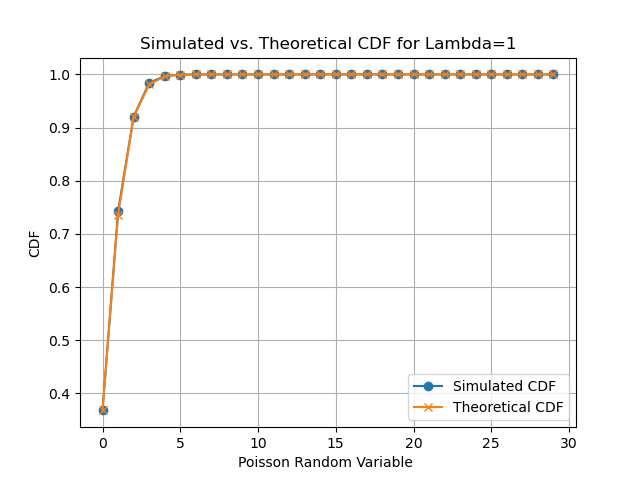
\includegraphics[width=\columnwidth]{2023/ST/56/figs/fig1.png}
\caption{CDF of X}
\label{fig:Theory vs Simulation}
\end{figure}
\begin{figure}[H]
\centering
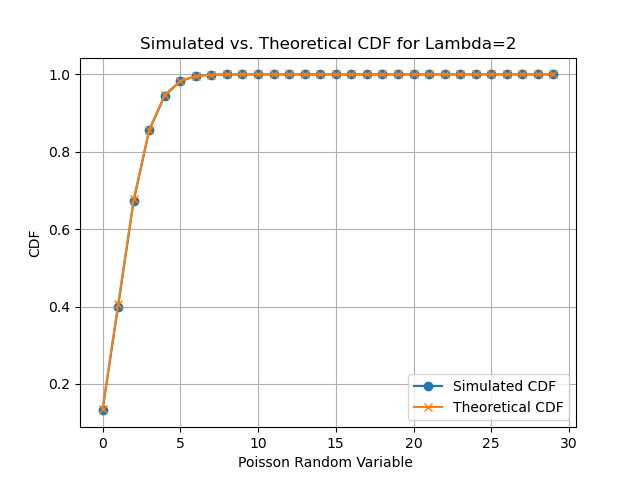
\includegraphics[width=\columnwidth]{2023/ST/56/figs/fig2.png}
\caption{CDF of Y}
\label{fig:Theory vs Simulation}
\end{figure}
